\chapter{Sources of Intelligence}

\note{introduction to cyber situational awareness tools was skipped}

\section{Connection to Cyber Sensors}
If we are to connect two systems to exchange data about assets (the same applies
to threats, vulnerabilities, etc.) we have to agree on:
\begin{itemize}
	\item What is an asset and what features and properties does it have
	\begin{itemize}
      \item From a format perspective
      \item Syntactically
      \item Semantically
   \end{itemize}
	\item How to exchange that data in an automatic and standard way between any given systems
\end{itemize}

This leads to the definition of standards for elements characterization and exchange, such as:
\begin{itemize}
   \item SCAP - Security Content Automation Protocol
   \item STIX - Structured Threat Information eXpression
   \item Assets
   \begin{itemize}
      \item ARF - Asset Reporting Format
      \item AI - Asset Identification
      \item CPE - Common Platform Enumeration 
   \end{itemize}

   \item Vulnerabilities
   \begin{itemize}
      \item CVE - Common Vulnerabilities Enumeration
      \item CVSS - Common Vulnerability Scoring System
      \item CWE - Common Weakness Enumeration
   \end{itemize}
   \item etc\dots
\end{itemize}

\section{SIEM}
\begin{paracol}{2}
   SIEM stands for Security Information and Event Management. It is a system that
   collects and aggregates log data from many different sources, normalizes the
   data, correlates it, and then alerts based on rules and heuristics.
   
   \note{\begin{itemize}
      \item Splunk
      \item QRadar
      \item OSSIM
      \item AlienVault USM (old)
   \end{itemize}}
   \switchcolumn

   \begin{figure}[htbp]
      \centering
      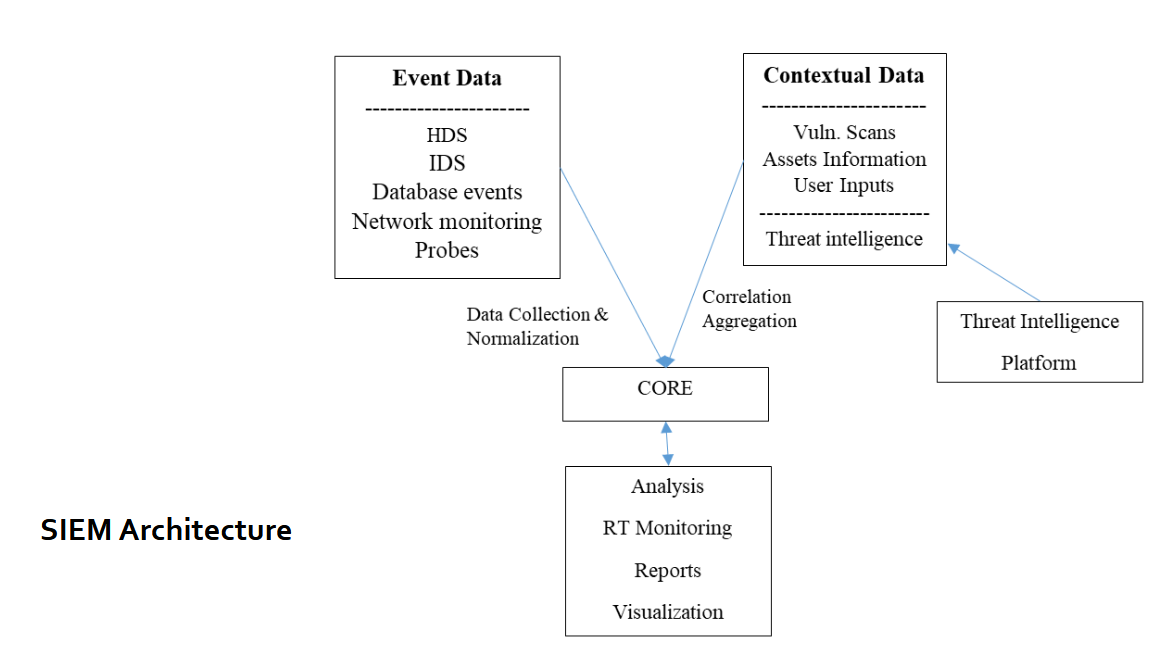
\includegraphics{images/04/SIEM.png}
      \caption{SIEM Architecture}
      \label{fig:04/SIEM}
   \end{figure}

\end{paracol}